\chapter{ReactJS}
\label{cha:ReactJS}

% one of biggest advantages is component based
% functional programming

In the previous chapter the application architecture Flux was introduced and discussed. Even tough aspects of this programming paradigm seem to be copied from other programming patterns, it is certain that Flux is not a bad application architecture after all. This section will demonstrate how Flux works best with Facebook's front end framework ReactJS (\cite{FacebookInc.2013}). The goal is to show the reader what is necessary to develop a web application by using cutting edge web technologies. This chapter will also provide an overview over some best practices and help the user to make application architectural decisions.

A few questions will come to mind: \enquote{What tools are needed to develop a \mbox{ReactJS} application?} or \enquote{Why should a web application programmer use this framework?}. Nowadays many large companies use JavaScript frameworks for the development of their web applications. The hard part in starting any web application project is to decide, which framework or technology is will be used. After reading this chapter all mentioned questions will be answered and it should be easier to make the right decision. This paper is \emph{not} a comparison between competing web technologies but it should give a clear overview of the features and benefits when using ReactJS.

\section{Why ReactJS?} \label{sec:whyreactjs}

As described in \cite[S.7-8]{Zeigermann.2016} there are several reasons why ReactJS is a good choice for a JavaScript front end Framework as described in the following paragraphs:

First of all, the framework is rather easy to learn and understand to get going and to simply start coding. There are some easy code examples \cite[Docs: Hello World]{FacebookInc.2013} to get started very easily. The difficulty is not very high even for programmers that do not have much experience at all. There is also always a link to a live coding website where basic ReactJS code examples can be tried out.

React's API is not extensive and well documented. The architectural decisions of the framework and the code of an application make it more easy to understand. Furthermore the ReactJS API hardly ever alters in a way that breaks already existing code. Facebook claims on many articles in their blog \cite[Blog]{FacebookInc.2013} that almost no time is wasted in refactoring deprecated ReactJS code from any outdated application. Experience has shown that indeed there had not been any situation where any front end specific code of ReactJS broke by updating to a newer version of ReactJS. If some component is about to be deprecated, it is clearly communicated on the release notes on the blog or by runtime development deprecation warnings that link to migration guides. 

ReactJS is a view-only framework. As stated on the project's starting page \cite{FacebookInc.2013}, Facebook does not make any assumptions about the development stack of the programmer. It is completely up to the software engineer to choose what technologies to use in conjunction with ReactJS. There are very few requirements from the framework itself. For instance it is totally up to the developer how to handle routing, application state and the communication to an API. That is also the reason why this framework appears to be very professional, as it is the programmer's responsibility to develop an application architecture and to choose the suiting development tools to tailor the application to the client's needs.

The ReactJS framework exists since the year 2013. During the time of its existence many technologies have been developed that work really well with this framework. Being highly component oriented it is possible to easily integrate third party ReactJS components from other developers. Custom ReactJS components are open source most of the time and can be integrated into any ReactJS project by using some form of a package manager. For example there are high-performance list or table views with lazy loading that optimize handling large amounts of data. Integrating those components can save a lot of time and improve the application's performance without the developer having to implement complicated components by him- or herself. 

Another advantage in developing ReactJS applications is that this framework has been in use long enough so there are many excellent developing tools available at the programmer's disposal. Everything from performance benchmarking tools to ReactJS component explorers can be integrated in any \mbox{ReactJS} project. One of the most important pieces of developing tools would be the possibility to automatically recompile and reload the application when files change without loosing the application state.

ReactJS is often compared to other frameworks in terms of performance and scalability. There is no definite answer which framework is the best amongst them of course. The fact that not only Facebook itself uses the framework but also other well known large well known companies like AirBnB\footnote{https://www.airbnb.com} or Plex\footnote{https://plex.tv/} as well provides good evidence that the framework can be well performing and scalable if implemented correctly.

% It should be mentioned that ReactJS is not only used by Facebook. Other well known large companies like AirBnB or Plex use the library as well. This is good evidence that the framework can be highly performant and scaleable if implemented correctly. 

\section{Introduction to the tooling for ReactJS}

When developing a \mbox{ReactJS} application, it is of utmost importance to understand all the tooling that is necessary to develop a ReactJS application. The technology which is necessary to transform \mbox{JavaScript} code into a code bundle that can be interpreted by the browser should not be a \enquote{black box} to the developer. When talking about a \mbox{ReactJS} application it often implies that the term \enquote{single paged application} is clear to the programmer as well. This section will explain all those terms and all necessary tools to create such a single paged application by using ReactJS.

%%here it should be stated why any sane person would go through the process of insane JavaScript npm or webpack processes to develop a web application.

\subsection{ECMAScript and Babel}

%here i will explain how to use stage-0 features of the JavaScript language that don't even have an implementation yet and why one would want to use these features.

\mbox{ECMAScript}\footnote{https://www.ecma-international.org} or ES for short is a specification for scripting languages and also specifies the scripting language \mbox{JavaScript}. \mbox{ECMAScript} is developed by \mbox{ECMA International}. Because \mbox{JavaScript} is a scripting language it needs to be interpreted by a JavaScript engine. The problem is, that ECMAScript is only a specification and different engines implement different versions of ECMAScript. Oftentimes clients demand application compatibility for older browsers like the Internet Explorer 11 for instance. The browser only supports only 11\% of the ES6 standard as this compatibility table\footnote{https://kangax.github.io/compat-table} shows. 

The following question arises: \enquote{What can be done if the web application that is coded in ES6 also needs to run on IE11?} \mbox{Babel}\footnote{https://babeljs.io/} is a JavaScript compiler, that transpiles JavaScript to JavaScript. This is especially useful in situations where the developer uses a version of the ECMAScript standard, that not all target runtime environments yet support. Currently almost all JavaScript projects use the \mbox{Babel} compiler to get the greatest compatibility across all runtime environments. The developer simply needs to select the desired ECMAScript version and \mbox{Babel} transpiles all JavaScript code to that specified version. It must be mentioned that not all features of modern ES specifications can be transformed to older ES versions.

The \mbox{Babel} transpiler not only transforms JavaScript to JavaScript but can also polyfill JavaScript features. A polyfill is a piece of code that implements a language feature that is considered native by the developer. For instance, the ES6 standard defines a function \texttt{Array.of()} that creates an Array object of a variable number of arguments. Internet Explorer 11 does not support this function, thus it needs to be polyfilled by babel so the browser can interpret the \texttt{Array.of()} function. If the function wasn't polyfilled, an error would occur and the application would crash. 

\mbox{ReactJS} works very well with modern ECMAScript features and proposals that are not yet implemented in many browsers. That is the reason why \mbox{Babel} is a very important developer dependency in almost any web project that uses modern JavaScript. As the development of JavaScript engines progresses, some time it will be possible to use a more recent ECMAScript version natively in the browser. With Babel the programmer just has to alter one line in the \mbox{Babel} configuration file to switch the transpiling target from ES5 to ES6 for example.

Especially for ReactJS, Babel is very important as it also transforms React's template language JSX into vanilla JavaScript. React can be used without JSX of course but it is not advisable as JSX is one of the most useful features of ReactJS highly increasing productivity and also adding a very useful abstraction layer to the framework. There will be an in-depth description of JSX in Chapter \ref{ssec:jsx}.

\subsection{NodeJS and NPM}

%here i will explain the best part of developing JavaScript applications with the Node Package Manager.

One of the biggest benefits of developing a JavaScript web application is the fact, that developers can use the node package manager npm\footnote{https://www.npmjs.com/}. This package manager allows the programmer can easily integrate any package or module into the web application. With a simple command \mbox{ReactJS}, \mbox{\mbox{Babel}}, \mbox{Webpack} and all the other necessary tools can be easily downloaded and installed without worrying about any dependencies. There are other package managers as well but npm is the most widly used JavaScript package manager. When installing NodeJS on a machine, npm is bundled in the installation. 

NodeJS\footnote{https://nodejs.org/} is not absolutely necessary for developing a React application, but \mbox{Webpack} offers an implementation of a development NodeJS server, that can automatically hot-reload React applications. This makes the developing process for web applications much faster and easier. In fact, developing a React application without NodeJS would be very inconvenient but possible after all. A bundled React application can be hosted on any static content serving web server. If the routing is configured correctly it is even possible to start the application directly from the file system as well.

\subsection{Webpack}

\begin{figure}
  \centering
  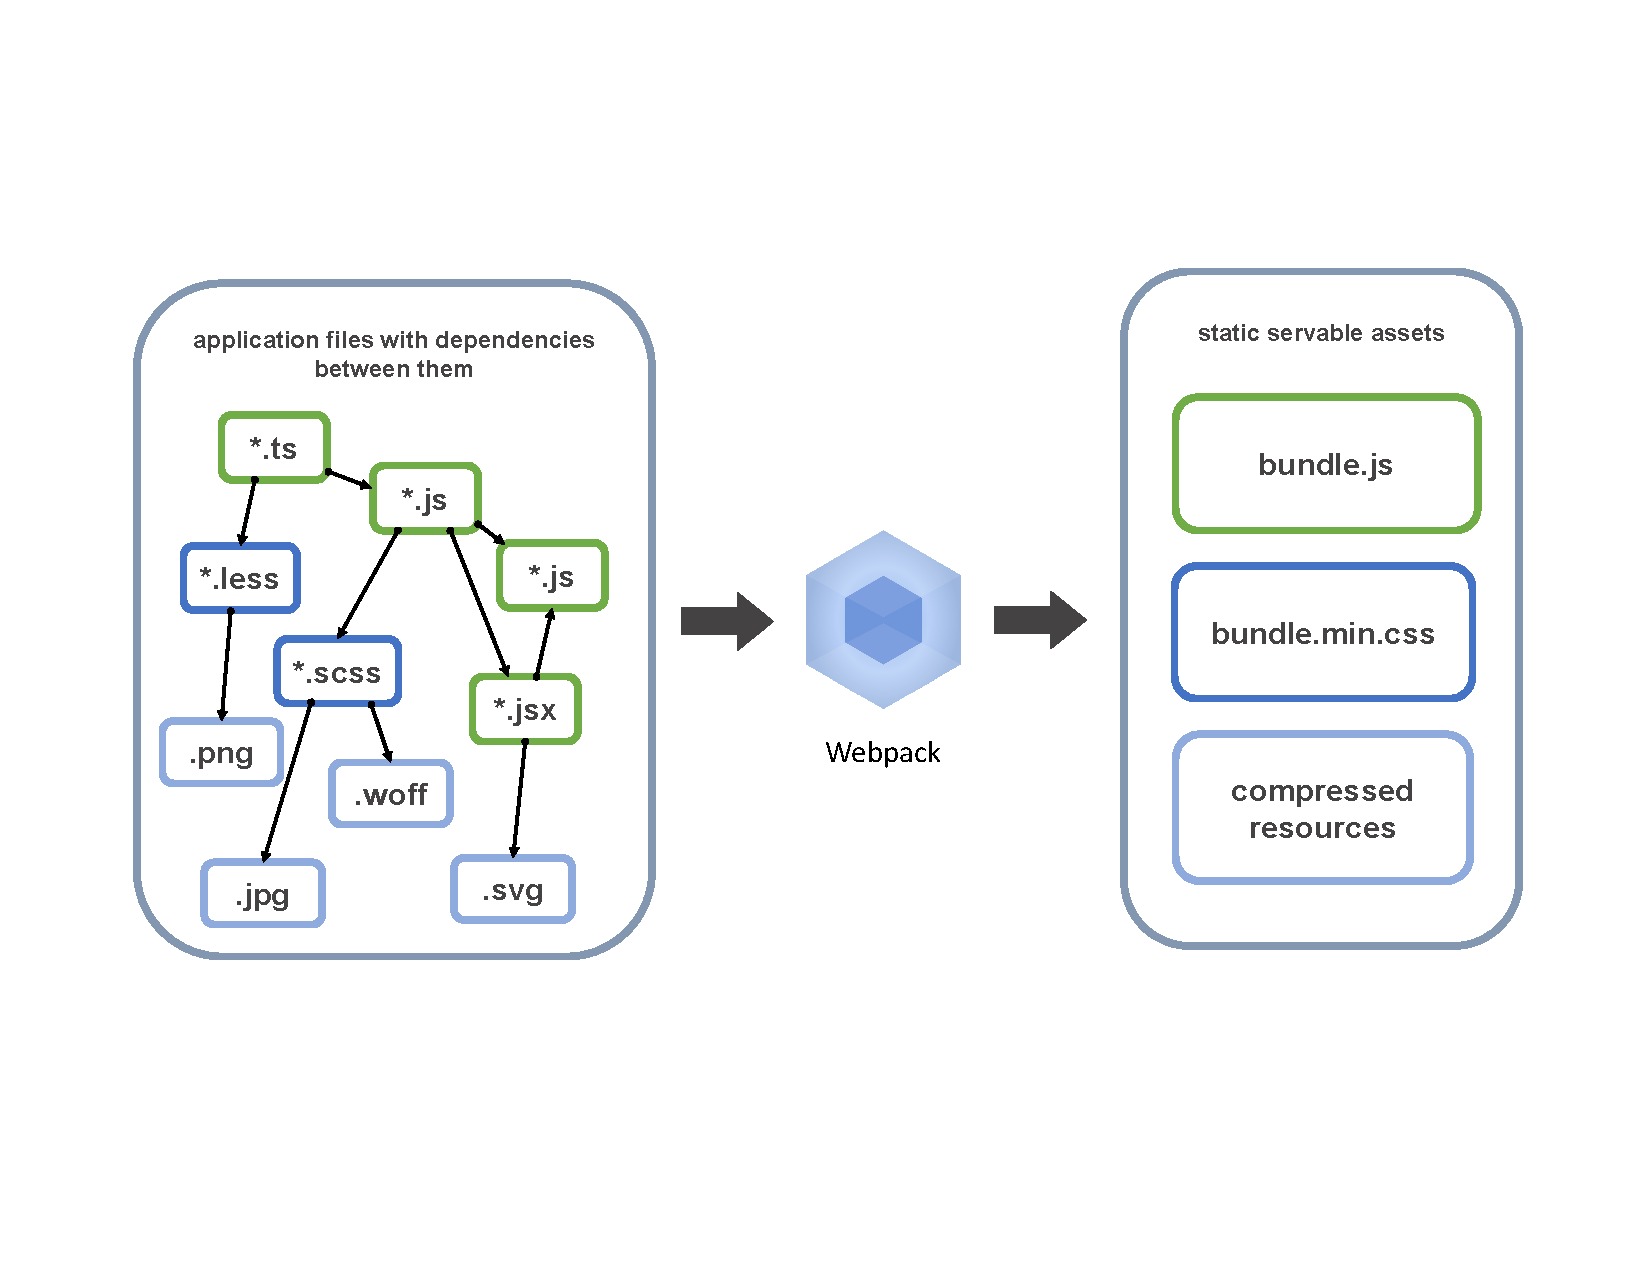
\includegraphics[scale=.6, trim= 2cm 4cm 2cm 4cm, clip]{007webpack.pdf}
  \caption{Webpack transformation visualization}
  \label{fig:webpack}
\end{figure}

\begin{figure}
  \centering
  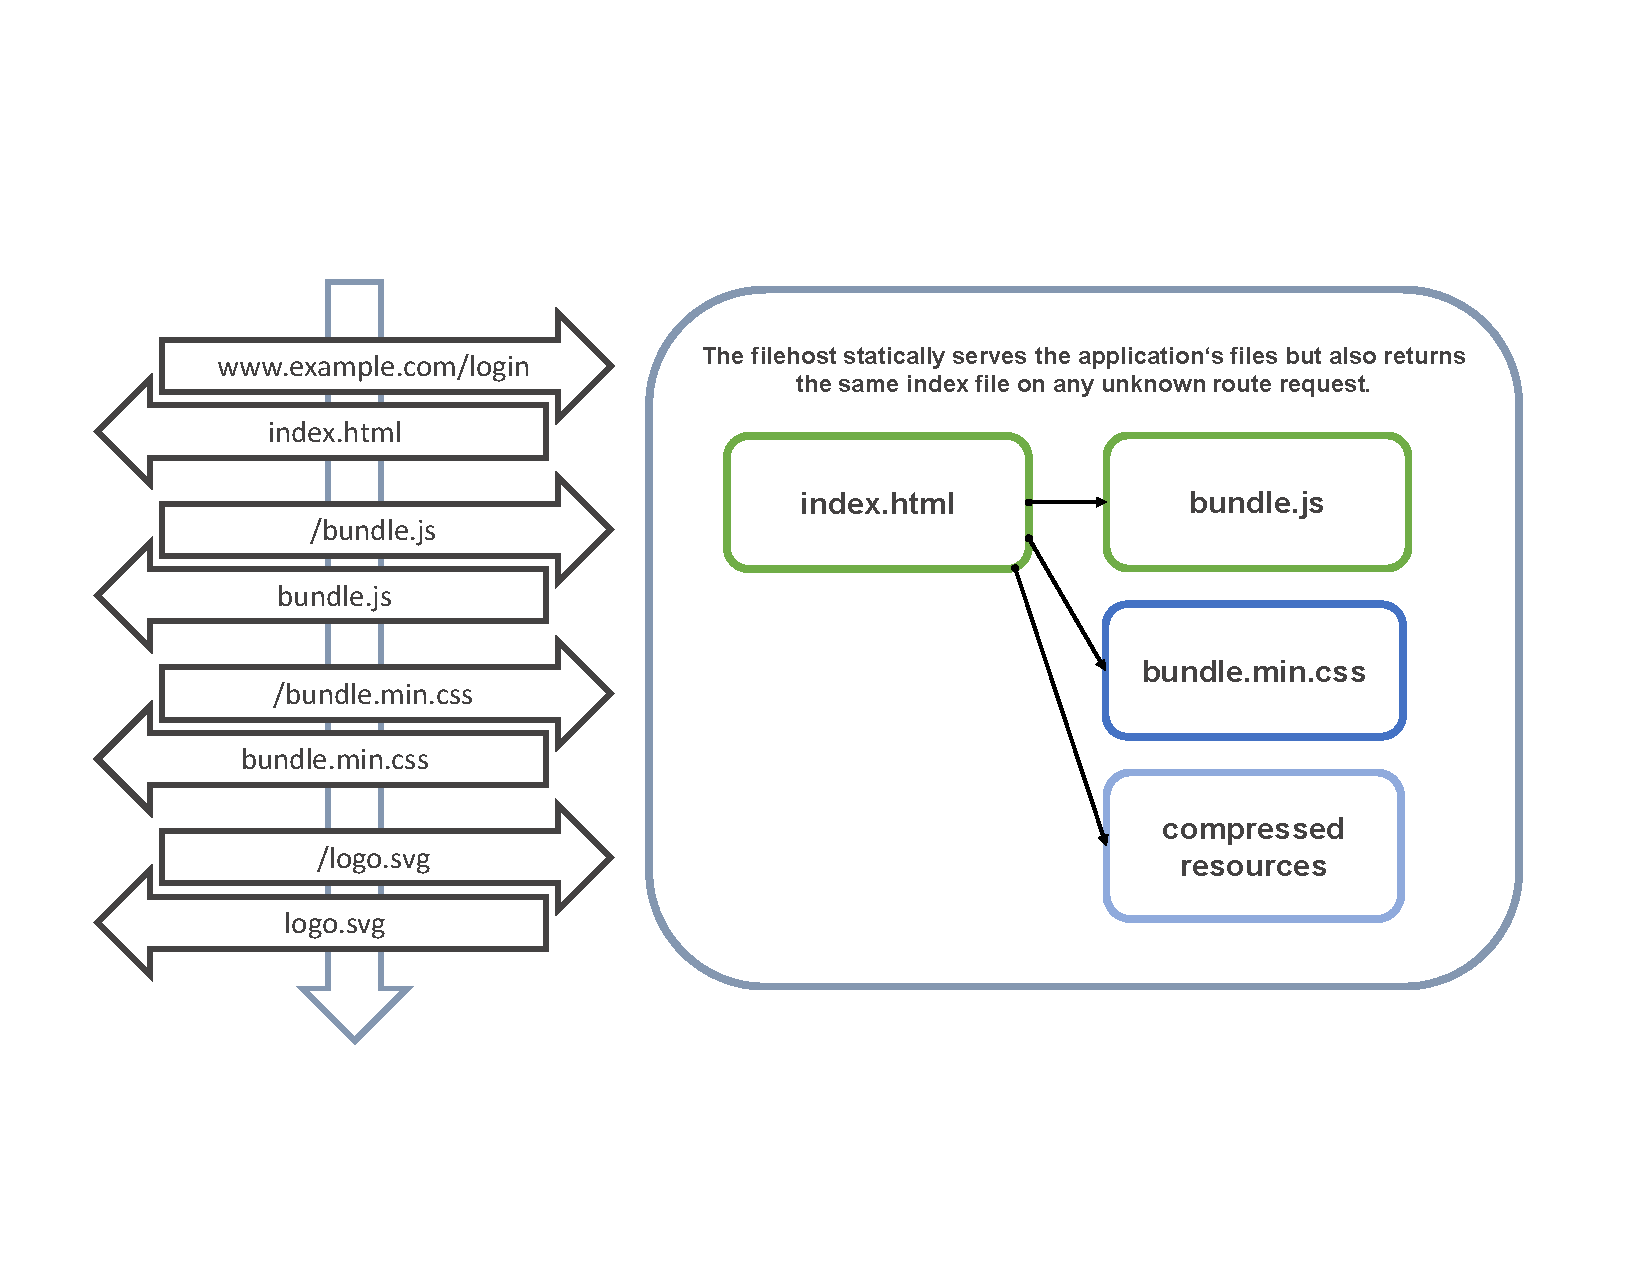
\includegraphics[scale=.6, trim= 1.5cm 3cm 2cm 2cm, clip]{008singlepagedapplication.pdf}
  \caption{Single paged application example}
  \label{fig:singlepagedapplication}
\end{figure}

\mbox{Webpack} is one of the most comprehensive developer tools that can be used for developing a web application using all kinds of files and language flavors. It is a module bundling mechanism that combines all the code base of a project into an application that can be interpreted by a browser. It does not matter if Less, Sass or plain CSS is used, neither does it matter if the project is developed in CoffeeScript, TypeScript or plain JavaScript. \mbox{Webpack's} base functionality is to transform modules with dependencies into static assets as described on the technology's website\footnote{https://webpack.github.io/} and as the example Figure \ref{fig:webpack} shows. 

\mbox{Webpack} is especially useful in combination with the Node Package Manager. Every module that was downloaded by npm can be integrated into the web application with a simple import statement and \mbox{Webpack} does all the work to integrate the module's code into the final bundle. \mbox{Webpack} will handle any dependency in the code and transform it into a code bundle, that includes not only the application's code but also third party module code, that was imported by the developer.

Another outstanding feature is the code splitting and the on-demand-loading of code. Not only is the code bundled and transformed into static assets but also split into code modules again in an intelligent way. Modules that are more heavily used in the application will be loaded first and other less important module parts can be loaded on demand. To avoid client side caching it is possible to include a generated build hash into the modules' name so the browser interprets each module as a new asset that is not yet cached. Deploying updates to an application is therefore no problem.

Many features can be accomplished with \mbox{Webpack} itself, but on top the module bundling mechanism is highly customizable as well. Webpack does support a plugin and loader system that can accomplish even more customization and variety in code transformation. Loaders can load, transform and then return any resource of the code of a web application. An example would be the loading of Sass files and the transformation to CSS. Another use for loaders would be the integration of image files. In the process of loading the images they can also be compressed and are output as static resources. Plugins on the other hand add useful features. One of the most important Plugins for development and production is the \mbox{DefinePlugin}. This piece of code allows the substitution of constants in the application's code according to the environment. With the help of this plugin the app can be run in development or production mode. There are several loaders and plugins provided by the Webpack community that can be downloaded and integrated by npm.

One of the most important features of Webpack for developing React apps is it's own development server. As stated before, NodeJS allows the developer to start a development server, that hot-reloads code parts so the developer does not have to recompile the whole code again in order to see the updated application after a change in the application's code. Not only NodeJS, but especially Webpack enables this feature. The code bundling mechanism enables watching file changes in order to compile changes on the fly and deploy them while the server that serves the front end code is still running. Again, this feature works with any asset of the app, whether it is a CSS file that has changed or a JavaScript file, the hot-loading mechanism is triggered.

When transforming a web application project with Webpack, the outcome is called a single paged application. The term describes a certain kind of web application that is started from one single index file. Most of the work is done by Webpack itself as it already transforms the web application's code into static assets. The server then only has to statically serve all application relevant data. If the requested route does not reference a static asset it means that the client must be requesting a certain page of the web application. In that case the server always has to serve the same index file. By doing that, the requesting client is guaranteed to always get the special index file that bootstraps the whole web application. The application can then react to the current route and display the correct page. The Figure \ref{fig:singlepagedapplication} shows how a request of the login page in a single paged application could look like.

%here i will explain what a one page application is, and how code bundling works with JavaScript imports and so on.

\section{Introduction and overview of the Framework}

Now that it is clear what is needed to set up a ReactJS project and there is a better understanding how the tooling works it is now time to dive deeper into the framework itself. This section will give an introduction to ReactJS and its history. Also basic application architecture will be discussed as well as conventions how to program a ReactJS application. Some core components of the framework will be described to achieve more knowledge on how the library works. 

To begin with, the JavaScript library ReactJS was developed by Facebook. The framework is open source since 2013 but it is still managed by technical engineers of Facebook and is available under a BSD license. The framework itself alows highly component orientated application architecture, which means code parts of a ReactJS application can be used in a very modular way. Once all the boilerplate code is built up and all standard components are implemented, big progress can be achieved in a very short amount of time. The most time consuming part of starting a React web application is to set up all the tooling and all the boilerplate code. To get a better understanding of the framework, some of its components will be explained to then show how a ReactJS application architecture could look like.

Where ReactJS really excels is when it comes to new web technology. The fact that the framework is a descriptive UI defining top-level API makes it easy to use ReactJS for other platforms and technologies as well. When developing a React application top-level highly abstracted simple components can be used that finally get broken down to library function calls that actually create UI elements. ReactJS could be described as a general user interface component abstraction library. Because ReactJS was engineered that way it is easily possible to use React to not only develop web applications but also to use React to develop mobile applications (React Native\footnote{https://facebook.github.io/react-native/}) or build virtual reality environments (React VR\footnote{https://facebook.github.io/react-vr/}) without much effort and without having to learn any new frameworks or programming languages. 

\subsection{JSX} \label{ssec:jsx}

As it can be read in \cite[S.59]{Zeigermann.2016}, \mbox{ReactJS} is a front end framework that does not need a template language to create user interfaces. Instead, the library provides functions to create or manipulate the actual DOM elements of a React component. To make the process of creating elements easier, ReactJS provides a JavaScript language extension called JSX. Code that is written in JSX can be transformed into JavaScript code by \mbox{Babel} and \mbox{Webpack}. 

Using the JSX language extension allows HTML-elemnts to be directly written into the JavaScript application code as this simple example shows. Note that it is necessary to use the JSX notation \texttt{className} instead of \texttt{class} as this is not vanilla HTML. All provided code examples can be tried out in any online live JavaScript editor\footnote{http://codepen.io/gaearon/pen/rrpgNB?editors=0010}. \newline

\begin{JsCode}
const HelloElement = (
  <div className='hello-world'>
    <span>I am a span</span>
    Hello World
  </div>
)
\end{JsCode}

The provided code snippet could not be interpreted by any browser and needs to be transpiled into vanilla JavaScript. The best part about JSX is, that components that are transformed this way are infinitely nestable. Components are easily and infinitely composable that way. ReactJS is a highly component oriented front end framework as mentioned before, making it easy to compose any ReactJS components. After the transformation the code looks like the following code snippet: \newline

\begin{JsCode}
var HelloElement = React.createElement(
  'div',
  { className: 'hello-world' },
  React.createElement(
    'span',
    null,
    'I am a span'
  ),
  'Hello World'
);
\end{JsCode}

The example shows, that the pseudo JSX DOM-elements are transformed into functions from the ReactJS API. The reason why components are infinitely nestable is that they get transformed into plain JavaScript functions that are composed as it can be observed in the example above. Using the functional programming paradigm composition makes it easy to compose any components. The return type is not an actual DOM-element, it is just a lightweight ReactJS JavaScript object but this fact is described in the Section \ref{ssec:VirtualDom} in greater detail. JSX can be tested with any online JSX transpiler like the babel transpiler for example\footnote{https://babeljs.io/repl/}

JSX is one of the most important features of ReactJS because it adds a very important abstraction layer to the view. The developer can use ReactJS components as normal DOM components without knowing the exact implementation. This is also the reason why ReactJS cannot only be used in the web but also for mobile platforms by simply switching the HTML components for the according components of the target platform. An example would be React Native which produces native apps for Android and iOS by using components like \texttt{<View>} instead of the well known HTML element \texttt{<div>} for example.

\subsection{Components and properties}

JSX is not only used to create common HTML elements, it can also be used to make use of components that were programmed by the developer. These so called \enquote{React components} can be JavaScript classes that extend the React \texttt{Component} class or pure functions as described in Section \ref{ssec:PureFunctionalComponent}. There was also the approach to use the React class factory function \texttt{React.createClass()} to use OOP style components in JavaScript. As the ECMAScript introduced the class syntax the class factory function was deprecated as it is better to use native classes than functions that get used as classes with the help of their closure. In the most cases components are functions or classes that can be used as a JSX element as shown in this example: \newline

\begin{JsCode}
class Hello1 extends React.Component {
  render() {
  	return <div>Hello, World!</div>
  }
}

const Hello2 = () => <div>Hello, World!</div>
\end{JsCode}

Note, that the anonymus function is declared as a ES6 \enquote{fat-arrow function}. Basically the \texttt{Hello1} and \texttt{Hello2} variables act identically. When rendered, they show the exact same output but have no functionality attached to them. The following example shows, how the newly created React components can be used with JSX: \newline

\begin{JsCode}
ReactDOM.render(
  <Hello1/>,
  document.getElementById('container1')
);

ReactDOM.render(
  <Hello2/>,
  document.getElementById('container1')
);
\end{JsCode}

The name of the component object defines the JSX element name. The two ReactJS API functions (\texttt{ReactDOM.render()}) will search for elements in the HTML-DOM that are called \enquote{container1} and \enquote{container2} and render the two React components instead of them. Usually, the \texttt{ReactDOM.render()} function is only used once in a ReactJS web application as a bootstrapping mechanism to set one element as the application root so ReactJS can build its actual DOM tree onto the specified element. As mentioned before, ReactJS components are infinitely nestable so there only has to be one actual root element in the real HTML-DOM to bootstrap onto.

To add functionality to a component it can be accomplished by passing it so called \textit{props} and processing them with JavaScript component logic. Passing a prop is really easy in JSX:

\begin{JsCode}
const HelloComponent = (props) => {
  props.ownFunction('this will get logged')
	return (
 		<div>
    	<h1>{props.title}</h1>
      {props.text}
		</div>
  ) 
}

ReactDOM.render(
  <HelloComponent title='Hello' text='World!' ownFunction={console.log} />,
  document.getElementById('root')
);
\end{JsCode}

\begin{figure}
  \centering
  
\includegraphics{001HelloComponent}
  \caption{Output of rendering HelloComponent}
  \label{fig:HelloComponent}
\end{figure}

The output of this snippet of code can be seen in the Figure \ref{fig:HelloComponent}. A very useful feature of JSX is that also functions can be passed to a React component. This is very useful when nested child components have to trigger logic in their parent component.

\subsection{Stateful components in ReactJS}

The component logic is very important in React. Functionality can be added by adding member functions to ReactJS class components to manipulate received props and providing a view to the provided data. Like discussed before, there are React components that are functions but there are also React components that extend the class \texttt{React.Component}. These classes do have a lifecycle and their own component state which can be manipulated as well. These class components produce more overhead as React treats these class components as smart components with state and lifecycle that has to be handed accordingly. Class components should only be used where it is absolutely necessary to reduce overhead and improve performance.

Lifecycle methods are very important if the component has to handle any asynchronous task or if incomming props have to be mutated. All the available methods are documented in the official documentation \cite[Docs: React.Component]{FacebookInc.2013}. For example there are methods that get executed before the component is about to mount (\texttt{componentWillMount()}), when it receives its props (\texttt{componentWillReceiveProps()}) or when it is about to unmount (\texttt{componentWillUnmount()}). The most important lifecycle method is the \texttt{render()} method though. This method gets called when the component has received its props and state and is about to render the view to the user. According to the documentation, API calls should be handled in the \texttt{ComponentDidMount()} method. The reason for that is to improve user experience. All components should render with an initial state and update themselves accordingly when asynchronously fetched data arrives. Another very important lifecycle method is the \texttt{shouldComponentUpdate()} method. The purpose of this method is to being able to exactly define the data that has to change in order to trigger the \texttt{render()} function. By overriding this method performance can be increased greatly because unnecessary rerendering cycles of the component that would otherwise slow down the whole application can be prevented.

Class components also have their own state that can be mutated by the member method \texttt{setState()}. As mentioned before, Facebook claims ReactJS does not make any assumptions about the development stack. This does also include the fact that ReactJS does not assume that the developer uses any form of application state container by him- or herself. This is the reason why ReactJS class components can have their own state which is tied to all the lifecycle methods. When either the component's state or props change the component will go through the according lifecycle methods including the \texttt{render()} method and is therefore rerendered. Class components are also often called \enquote{stateful components}.

The following code example shows how a stateful component could look like. Note that it is still possible to pass props to the stateful component. React makes use of the ECMAScript class syntax and extends the \texttt{React.Component} base class for creating stateful React components.

\begin{JsCode}
class StatefulComponent extends React.Component {
  
  constructor(props) {
    super(props)
    // setting the initial state in the constructor
    this.state = {
      value: 'initial'
    }
  }
  
  mutateState(value) {
    // mutate state with React Component method to trigger lifecycle methods
    // this method is asynchronous
    // any asynchronous action can be performed like calling an api
    this.setState({ value })
  }
  
  componentDidUpdate() {
  	console.log('i was updated')
  }
  
  render() { 
    return (
      <div>
        <button onClick={this.mutateState.bind(this, 'mutated!!!')}>Mutate Me</button>
        <p>{ this.state.value }</p>
      </div>
    )
  }
}
\end{JsCode}

When executed, a button and a text field (paragraph tag) are shown. Initially the text renders as \enquote{initial}. Once the button is pressed, the internal state of the component changes and it renders \enquote{mutated!!!}. Every time any props or state changes, the React component reiterates all lifecycle methods that are implemented. In this example the \texttt{ComponentDidUpdate()} method gets executed after each time the button was pressed because the state of the component changed by executing the \texttt{setState()} method.

%% achitecture -> 

% maybe show an example of smart component?
% "smart" and "dumb" components

\subsection{Pure functional components} 
\label{ssec:PureFunctionalComponent}

The other type of components ReactJS has to offer are so called \enquote{functional components} or \enquote{stateless components}. This type of component is often used to render parts of the application that do not have any component logic attached to them. Functional components are only a declaration of how the component has to look at a certain state. These components receive the application state via props and can also trigger logic operations by invoking functions that were passed as props as well. Functional components are often called \enquote{dumb components} because their only reason of existence is to provide a view to a certain application state.

When seen in the perspective of functional programming one could also call these components pure functions. The fact that the functions are pure without any side effects make the components easily testable. Functional components are pure functions that will always produce the same view for the same constellation of props. React does \emph{not} treat these dumb components as a stateful component. That is the reason why there is no additional overhead as the JSX component gets transformed into a simple \texttt{React.createElement()} call as it can be seen in the examples above. Neither lifecycle nor component state has to be considered by React when using pure functional components which greatly improves performance and reduces script execution time overhead. 

The following code snippet is considered a functional component. Components like buttons or text input fields are perfect for being a functional component as they will get used very often throughout the whole application.

\begin{JsCode}
const FunctionalComponent = (props) => (
  <div>
    with the same props i will always render the same...
    {props.text}
  </div>
)
\end{JsCode}

The only constraint of functional components to be used in conjunction with JSX is, that they have a capital letter at the beginning so JSX recognizes the function as a React component. The component can then be used very easily in JSX as the following snippet shows:

\begin{JsCode}
<div>
  <FunctionalComponent text='I am so pure!' />
<div>
\end{JsCode}

% "dumb" components only function, only view

% \subsection{React Router}

% components with logic, after that only functional components
% routing of the app, hash routing, react router breaking changes every few months

% \subsection{Styling}

% is this really necessary, maybe covered in webpack section?

\subsection{Property Types}

JavaScript is a dynamic typeless scripting language. Because of this very reason ReactJS provides an API that lets developers specify property types for each component. When React is executed in the development mode each component will check the provided property types to ensure that the component is used correctly. The following example shows how the so-called \texttt{PropTypes} can be used:\newline

\begin{JsCode}
const Component = (props) => {
  
  // if the prop title is not set it gets set to a fallback value
  // the prop is not guaranteed to be set so the programmer has to implement a fallback
  const title = props.title || 'I am the standard title'
  
  // the callback property is guaranteed as it is set to isRequired
  // if the text prop is not set the defaultProps object will set it
  return (
    <div>
      <button onClick={props.callback}>Button</button>
      <p>{props.title}</p>
      <p>{props.text}</p>
    </div>
  )
}

Component.propTpyes = {
  title: PropTypes.string,
  callback: PropTypes.func.isRequired,
  text: PropTypes.string,
}

Component.defaultProps = {
  text: 'i am the default text'
}

\end{JsCode}

The \texttt{propTypes} and the \texttt{defaultProps} objects are static and can be assigned to statful \emph{and} stateless components. The \texttt{propTypes} can be used to specify which property has to be of what type and to specify which component is required. To read about the full potential of \texttt{PropTypes} it is advised to have a look at React's documentation (\cite[Typechecking With PropTypes]{FacebookInc.2013}). The \texttt{defaultProps} object can be used to set props to a default value if they are not set by the user of the component. By doing this the developer of the component does not have to implement fallback solutions if the property is undefined.

It is important to note that the property check is disabled when ReactJS is bundled in production mode as the type checks are only viable during the development of the application and introduce scripting overhead. The default properties on the other hand get set even when the production mode is enabled.

\subsection{Virtual DOM} 
\label{ssec:VirtualDom}

% makes react very fast
% dom operations expensive
% javascript object light weight and fast
% diffing algo and reconciler
% renderer pluggable

The most expensive operations when it comes to rendering anything in the browser are DOM manipulations by JavaScript. React solves this problem by using a concept named \enquote{Virtual DOM} or \enquote{shadow DOM}. As stated in \cite[Docs: Reconciliation]{FacebookInc.2013} ReactJS is a declarative framework that allows the user not having to think about the changes that have to applied to the current built up DOM elements. When using frameworks like jQuery, DOM elements have to be referenced directly in order to manipulate them. ReactJS on the other hand builds up its own Virtual DOM which is a plain old JavaScript object, calculates any changes with its built in diffing algorithm and applies possible changes to the DOM making the framework very fast. Instead of having to tell the browser what elements to update it is possible to tell React how the application should look like at any given state (declarative) as it can be heard in \cite[1:50]{youtube.2017}. This mechanism is called the \enquote{reconciliation algorithm} and is a part of the core algorithm of React.

Internally using a Virtual DOM is not only useful in the web where there is an actual DOM but also in other hardware environments as stated in \cite[2:10]{youtube.2017}. Facebook decided to divide the diffing algorithm and the part of the code that actually handles pending changes in the DOM which led to the distinction between the \enquote{renderer} and the \enquote{reconciler}. The renderer was transformed into a pluggable part of ReactJS enabling the framework to be available on other platforms as well. React Native for example is a ReactJS framework that makes it possible to produce mobile applications that can be compiled for Android and iOS by simply switching out the renderer part of the ReactJS core algorithm.

% \subsection{React Fiber} \label{sec:reactfiber}

% talk about how virtual dom is outdated and fiber will win

\section{Redux}

In Chapter \ref{cha:fluxreduxmvc} the programming pattern Flux was introduced. In the early days of ReactJS, Flux had to be implemented by the developers themselves because there was no framework that could handle application state management by using the Flux pattern at the time. To encourage developers to use the Flux pattern the Redux framework was born in May 2015 which can be researched in \cite{DanAbramov.2015}. The library is basically a state container that is designed with the Flux application architecture in mind. Redux can be used for any application but it suits very well to be used in conjunction with ReactJS. If the reader decides to utilize the Flux architecture to program a web application, it is definitely a good idea to use Redux. The library makes it exceptionally easy to develop an application with the new paradigm in mind and takes the overhead of having to design a Flux architecture by the programmer away.

% what is redux and why does it exist and how does it make web development easier

\subsection{Introduction and overview} \label{ssec:introductionoverview}

With Redux it is very easy to implement a global state on any front end application. Like the Flux design, Redux also consists of components like the Action and the Store component with a Dispatcher handling incoming actions. Redux is a little bit different than Flux though. Like explained in the Section \ref{ssec:fluxstore}, Flux can have multiple stores that can be registered via a callback. Redux only has one store and achieves this by composing all stores into one store. The goal is, that actions can be dispatched onto the store resulting into a mutated state that can then be set and passed to any connected ReactJS component.

% describe actions with code example
Like described in Section \ref{ssec:fluxaction}, an Action can be created by any user interaction and has to be dispatched to the store. As it can be read in \cite[Actions]{DanAbramov.2015} an action has to return an Object containing all necessary information for the reducer which will be introduced in the next section. An example of an Action could be the following code snippet:

\begin{JsCode}
const mutateStoreData = (data) => {
  return {
    type: MUTATE_DATA,
    data,
  }
}
\end{JsCode}

As per default, it is rather complicated to perform asynchronous operations in an Action. The documentation \cite[Async Actions]{DanAbramov.2015} suggests to use a middleware (redux-thunk\footnote{https://github.com/gaearon/redux-thunk}) that allows actions to have a callback to perform asynchronous actions. An example could be the following code snippet:

\begin{JsCode}
const asyncMutateStoreData = (params) => (dispatch) => {
  doSmthAsync(params, (error, data) => {
  	// this is the callback function context of doSmthAsync 
    // it gets called once the async operation is complete
    // this could be a file system operation or an API call
    if (error) throw new Error('error')
    // the dispatch callback can be used to resolve asynchronously
    // data from the action can be dispatched to the store at any point in time
    dispatch({
      type: MUTATE_DATA,
      data,
    })
  })
}
\end{JsCode}

The so called \enquote{Reducer} is a very important aspect of Redux as it can be read in \cite[Reducers]{DanAbramov.2015}. The reducer is responsible for taking the store's data, changing it by using a pure function that takes the current state and an action and returns the newly calculated state. It is of utter importance to understand, that the state is \textbf{not} mutated. The newly evaluated state is then set as the new current global state. This makes applications very easy to debug because there are no side effects in the reducer as it is a pure function. There is even a tool\footnote{https://github.com/gaearon/redux-devtools} which can restore any previously set states of the store, creating the possibility to \enquote{time travel} through all different versions of the application state. It is exceptionally easy for the developer to restore any previously set state which increases the debugability of the application greatly.

The following code example shows how a reducer function could look like:

\begin{JsCode}
const reducer = (state, action) => {
  switch(action.type) {
  	
    case MUTATE_DATA:
      state.data = action.data
      return state
  
    default: 
      return state
  }
}
\end{JsCode}

% reducer code example
% maybe insert a graphic here?? or next section? maybe show redux dev tools?

\subsection{Connection to ReactJS}

Redux is very often used in conjunction with ReactJS. According to the statistics of Sacha Greif \cite[Front-End Frameworks]{SachaGreif.2016} about 60\% of developers that use ReactJS also use Redux for state management. To use Redux with React a package named \texttt{react-redux}\footnote{https://github.com/reactjs/react-redux} has to be used in order to connect React components to the Redux store. The react-redux package provides a \texttt{connect()} function that can be used to compose a React component that is intended to be connected to the store.

It was promised before to show why Flux-Redux works well with React. The reason why Redux is perfect for React is, that the application state is passed to a component as a prop. As the reader should know by now, React components only update when either props or the state change. Through the react-redux package certain parts of the state can be mapped to a component only causing rerenders when the corresponding prop that was mapped from the state changed.

The following code example shows how easy it is to map the stores state to a component. The \texttt{connect()} function takes a state mapping function as a parameter. The \texttt{connect()} function is composable and therefore has to be invoked a second time by passing in the component that has to be connected to the store. The first invocation of \texttt{connect()} returns a function that will take either a stateful or stateless component. The code example also shows how to dispatch an action to the store. When composing a component with the \texttt{connect()} function, the \texttt{dispatch()} function automatically gets added to the props of the connected component. \newline

\begin{JsCode}
const mapStateToProps = (state) => {
  const { dataToExtract } = state
  return { dataToExtract }
}

const MyComponent = (props) => {
  // this component can access the store's current state
  // every time the mapped state changes, this component will rerender
  return (
    <div>
      <button onClick={() => this.props.dispatch(mutateStoreData('mutated!!!')}></button>
      {props.dataToExtract}
    </div>
  )
}

// this is where the magic happens and where the component is connected
export default connect(mapStateToProps)(MyComponent)
\end{JsCode}

% CODE EXAMPLE with connect
% how can redux be connected to react js
% component tree updates

\subsection{Immutability of the store's data}

Probably the most important aspect to consider when using Redux with ReactJS is to use a library that makes the Redux's store data immutable. Immutability is a very complex topic when programming applications with JavaScript. As a developer you can never be sure what operations mutate the objects and what functions clone the object and return the mutated object as the function's result. There are several packages that can be used to make the store's data of Redux immutable, like the \enquote{seamless-immutable} package. These immutability libraries ensure the programmer that a JavaScript object created by any chosen immutability library cannot be mutated directly. It has to be done by using the libraries API or by creating a new object.

The question that arises is: \enquote{Why is immutability so important when using Redux?} The answer to that question is very simple: Once React applications get very big, performance can be a serious problem if too many rendering cycles happen at the same time. ReactJS provides an API to check if a component should be updated or not. This is usually handled by a shallow comparison of the objects or can be implemented by the developer by overriding the lifecycle method \texttt{shouldComponentUpdate()}. When mapping a whole component tree to the component, a shallow compare will not be sufficient to note any changes in the JavaScript state object if it was changed deep down in the object tree. The solution to this problem would be a deep compare but having to iterate the whole state object tree can be a very expensive operation in addition to a complete rerender of the component. 

If many state changes occur in a very short amount of time the comparing function has to be executed on every prop or state change. That is the very reason why the comparing function should be as performance efficient as possible. With an immutable object the comparison function can just directly compare the objects which is an extremely cheap JavaScript triple equals comparison. The object cannot be mutated by a simple JavaScript operation and once the state has to be mutated it has to be done by the immutability library or by creating a new object. Either one of these cases cause the JavaScript triple equals comparison to not return true therefore causing a rerendering cycle. If the previous and the current state object are equal the component knows that the state has not mutated and will not rerender.

In the Section \ref{ssec:introductionoverview} a code example of a possible reducer was shown. In that example the object is mutated directly by accessing a property of the store object. In JavaScript mutating an object by accessing a property does not mutate the whole object but only that property. To notice any changes the object cannot be compared by JavaScript's triple equals operator but one would have to write a deep comparison function comparing all properties of the object. When using immutable objects the object itself knows when it was mutated even if the mutation happened deep down in the object tree making the comparison with the triple equals operator possible again.

As the time of writing this, ReactJS is in the version 15.5.4. This version not only provides a \texttt{React.Component} base class to extend from, but also a \texttt{React.PureComponent} class that automatically implements the \texttt{shouldComponentUpdate()} method. This special component achieves this by automatically shallow comparing all current props with every new incomming prop. When using an immutable store this component type gets highly useful as the programmer does not have to implement the \texttt{shouldComponentUpdate()} method.

% \subsection{Asynchronous store}

% make javascript even more scalable by making even state changing actions async and let the script language engines decide when to execute the actions and thus increase performance

\subsection{Advantages and disadvantages of using Flux-Redux}

Probably the biggest advantage of using Flux-Redux in any React application is the possibility to store a global application state that lives as long as the user is actually using the web application. This can improve user experience greatly. A good example would be the possibility to being able to trigger a function that displays an error modal from any part in the application. The modal's state could be \texttt{\{ visible: true \}} which tells it to be displayed no matter what state the rest of the application is in and what screen component is displayed at the time of triggering the function. Another good example would be user input. The user inputs some form data but changes the view causing different components to be displayed. Once the user comes back to the form component the state is still saved in the Redux store.

A big disadvantage is the amount of boilerplate code that is necessary to create actions and reducing functions. Once the programmer decides to divide the application into more than one store all of these stores have to be somehow composed before they can be used by the Redux library. The framework has an API that lets programmers compose stores and middlewares but it is still boilerplate code that costs time.

Once there is a part of the app that needs to store state in any store several steps have to happen that cost time and programming overhead as well. First an Action has to be implemented that possibly handles API calls and prepares some data for the store. An action constant has to be created as well in order to being able to dispatch the action to the stores. The action constant is the action type that gets parsed in the store's reducer function to decide how to reduce the data. Finally, the corresponding reducing function in the store has to be implemented. Once all of these components are finished they somehow have to be connected to the ReactJS component that will utilize the newly implemented logic. As mentioned before, the package \texttt{react-redux} provides an API to compose any React component to be connected to the store. In order to being able to do this mapping functions have to be written that not only map the store's state to the components props but also maps the corresponding actions to the props of the component so that they can be used inside the component. The programming overhead can be considered as big disadvantage but it guarantees unidirectional dataflow, debugability, scaleability, and testability of the application.

%% any code examples of creating store? any graphs?

\section{Application Architecture} \label{sec:application-architecture}

Now that the reader is a more familiar with React's concept of stateful and stateless components and knows more about how to store application state efficiently it is time to talk about best practices to build well performing and scaling ReactJS web applications as promised at the beginning of this chapter. Of course there are no definite best practices, this paper is based on personal research and personal experience. The reader is invited to evaluate every suggestion him- or herself and form his or her own opinion.

In most cases it is the best practice to think about the fundamental application architecture before starting the project. The application should strictly be divided into smart and dumb components. Currently a community standard is arising that divides web applications into pages (smart components) that handle all the application logic that is relevant for the page and components (dumb components) that can be reused throughout the whole application. Good candidates for stateless components would be a button with a certain style attached to it or a component that can handle page layout. Instead of using native DOM elements every application should reach a point in time where the development of stateless components allows to construct a page by using only own components from the existing component directory.

If there is the need to use a stateful component use the \texttt{PureComponent} base class from the ReactJS API or the \texttt{shouldComponentUpdate()} lifecycle method. It is always a good idea to carefully consider what prop and state changes should cause the component to rerender. Nevertheless, using stateful components should be avoided where ever possible. The best practice would be to only have one parent component that implements all the component logic via member methods and passes them down to all children. The application is much easier debugable because there is only one component where logic is executed and where the data comes from.

Never map child components to the Redux store. The best practice is to only connect page components to the store and pass all relevant data and functions as props to the child components as mentioned before. By strictly following this best practice the structure of the application is much easier understandable and readable. The code base gets more maintainable as new contributors exactly know where all the logic operations happen and where data comes from. When also connecting child components to the store the code base can get very confusing and it is harder for the developer to prevent unnecessary component rerendering cycles.

\begin{figure}
  \centering
  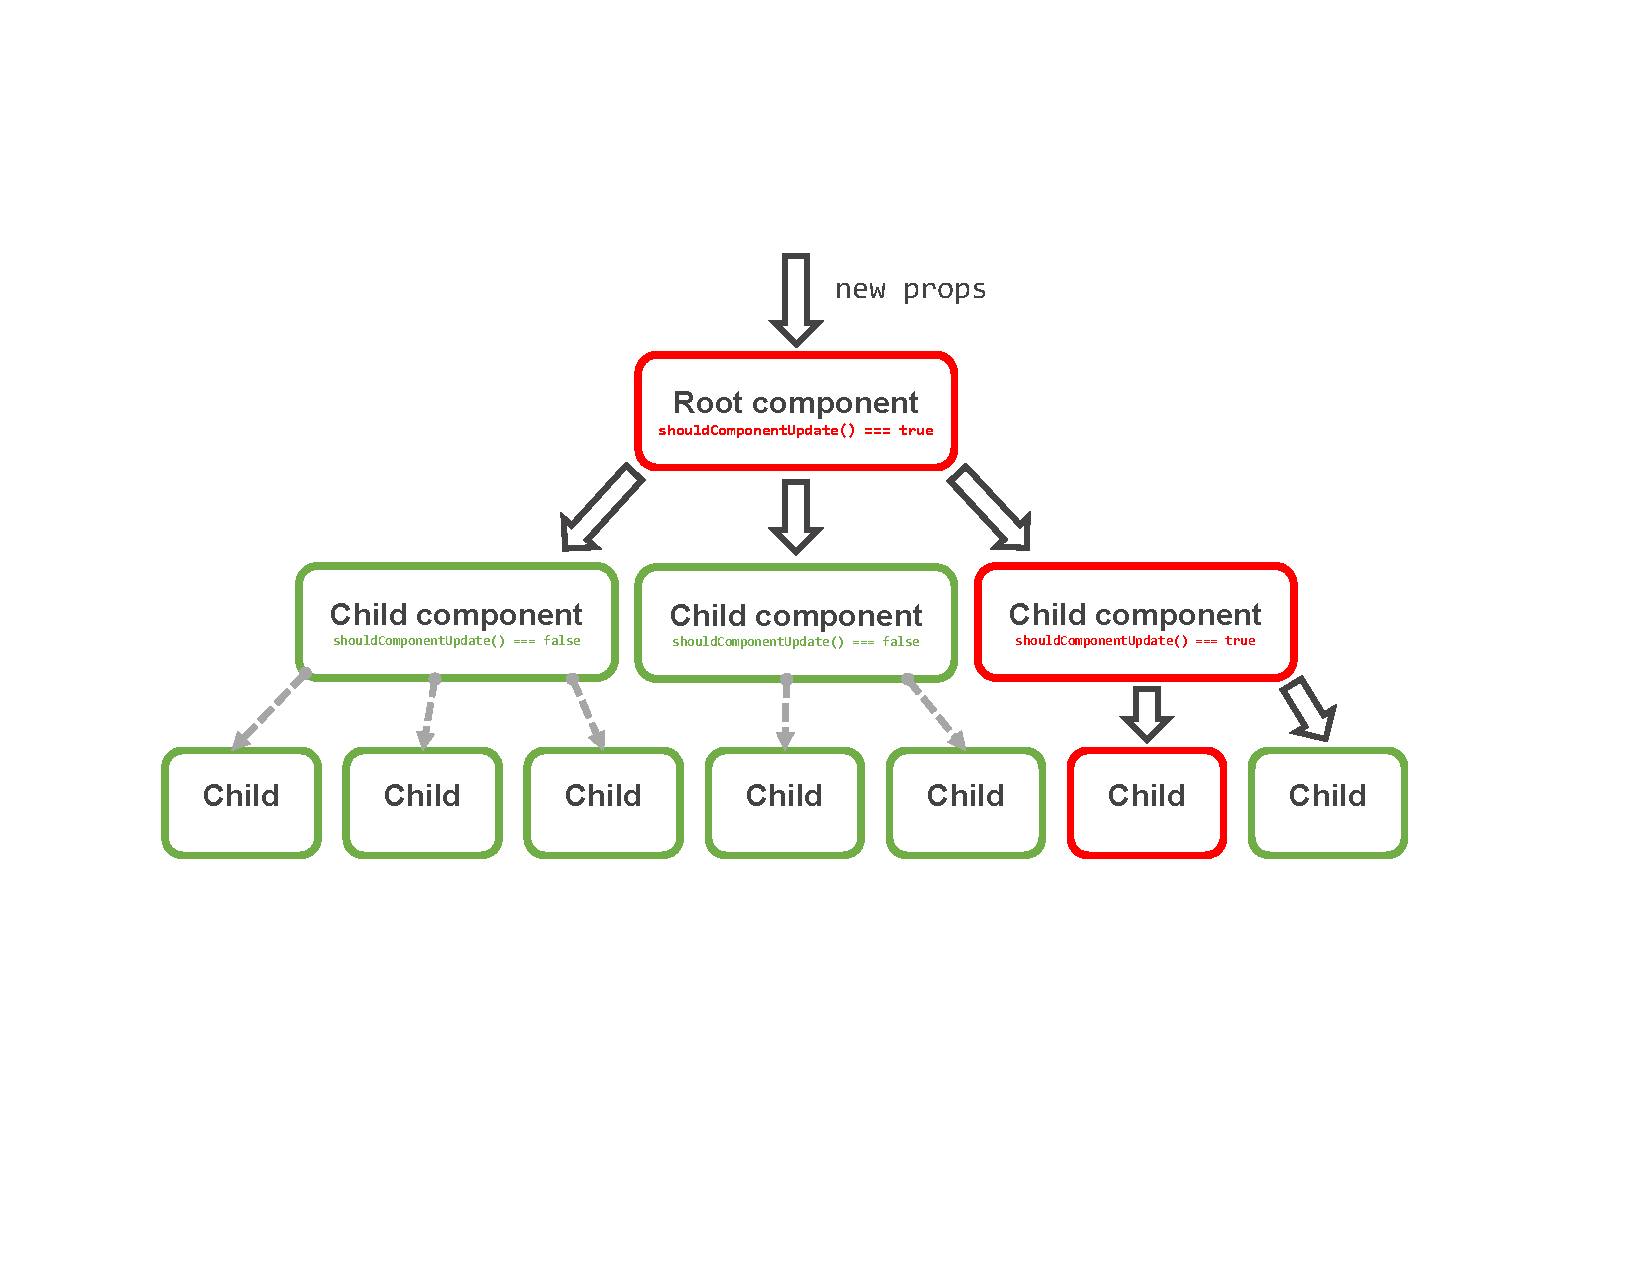
\includegraphics[scale=.7, trim= 2cm 6cm 2.5cm 3cm, clip]{009reactupdatecycle.pdf}
  \caption{React render cycle chain example}
  \label{fig:reactrerenderchainexample}
\end{figure}

Another advice is to split the application into logical component sections. In ReactJS child components only rerender if their parent components went through an update cycle thus changing the child component's props. To prevent massive rerendering chain reactions it is only necessary to prevent a parent component from rerendering (either by using React's base class \texttt{PureComponent} or by implenting the \texttt{shouldComponentUpdate()} method) and a side effect of this is that none of its child components will rerender neither as it can be observed in the Figure \ref{fig:reactrerenderchainexample}.

Use the new fat arrow syntax of ES6 as it makes the code look more clean and also resolves the problem of binding the correct context to utility functions that have to be passed to child components. The following code example will show the difference between the different approaches and how the code can be kept clean by using fat arrow functions: \newline

\begin{JsCode}
const ChildComponent = (props) => {
  return (
    <div>
      <button onClick={props.action}>will cause error</button>
      <button onClick={props.correctlyBoundAction}>will mutate state</button>
      <button onClick={props.oldWayOfBindingAction}>will also mutate state</button>
    </div>
  )
}

class ParentComponent extends React.PureComponent {
  
  constructor(props) {
  	super(props)
    // this is ugly boilerplate code
    // it was necessary before fat arrow functions were introduced with ES6
    this.oldWayOfBindingAction.bind(this) 
  }
  
  action() {
    // when executed in the child component this is undefinded -> error
  	this.setState({ value: 'mutated' })
  }
  
  correctlyBoundAction = () => {
    // through the arrow function the this context is correctly bound to the function
  	this.setState({ value: 'mutated' })
  }
  
  oldWayOfBindingAction() {
    // this context is bound in the constructor
  	this.setState({ value: 'mutated' })
  }
  
  render() {
  	return (
      <div>
      	<ChildComponent
          action={this.action}
          correctlyBoundAction={this.correctlyBoundAction}
          oldWayOfBindingAction={this.oldWayOfBindingAction}
        />
      </div>
    )
  }
}
\end{JsCode}

Experience shows, that sometimes it makes sense to swap out functional components with classes that extend the \texttt{PureComponent} base class. It makes the component a stateful component that has to go through all lifecycle methods but in some cases where a big amount of data has to be passed to a component or the component is expensive to render it sometimes makes more sense to use a \texttt{PureComponent} than a pure function to prevent unnecessary rerendering cycles.

It is strongly advised to implement the \texttt{propTypes} object of every component. By doing so the application is easier to understand for developers that are new to the code base. Developers who want to use or debug any specific component can easily check what properties exist for the component and what properties are mandatory to being set. This increases the process of understanding each component's logic even if the code is rather complicated.









